\setcounter{chapter}{4}
\setcounter{section}{0}
\part{RESULTADOS Y DISCUSIÓN} 

\section{Resultados de la metodología}

Los resultados que se obtuvieron al aplicar la metodología basada en el manifiesto del desarrollo de software ágil se redactan a continuación:

\subsection{Análisis de requisitos y obtención de pruebas}

Para llevar a cabo el análisis de los requisitos sobre la librería JavaScript que se desarrolló se tomaron en cuenta varios favores observando las carencias que existen al momento de realizar el modelamiento de cualquier software. Mediante el docente encargado de impartir las clases sobre cómo utilizar los lenguajes de modelado como lo es UML se dio cuenta que podría existir una forma en generar uno de los diagramas más importantes que es el diagrama de clases, pero a partir de las descripciones que se generan en los casos de uso del sistema.

Existe una herramienta denominada TDDT4IoTS que permite realizar el modelamiento de varios tipos de software. La herramienta cuenta con un lenguaje de símbolos que permiten escribir dentro de las descripciones de casos de uso datos técnicos sobre los objetos que intervendrán en el sistema informático que llevara a cabo la ejecución de todos los escenarios que se están describiendo. A petición del cliente recomendó que visitemos el sitio web de aplicaciones.uteq.edu.ec/tddt4iots para visualizar  los símbolos que usa la herramienta (ver figura \ref{fig:simbolostdd}).

\begin{figure}[H]
	\caption{Símbolos que utiliza la herramienta TDDT4IoTS}
	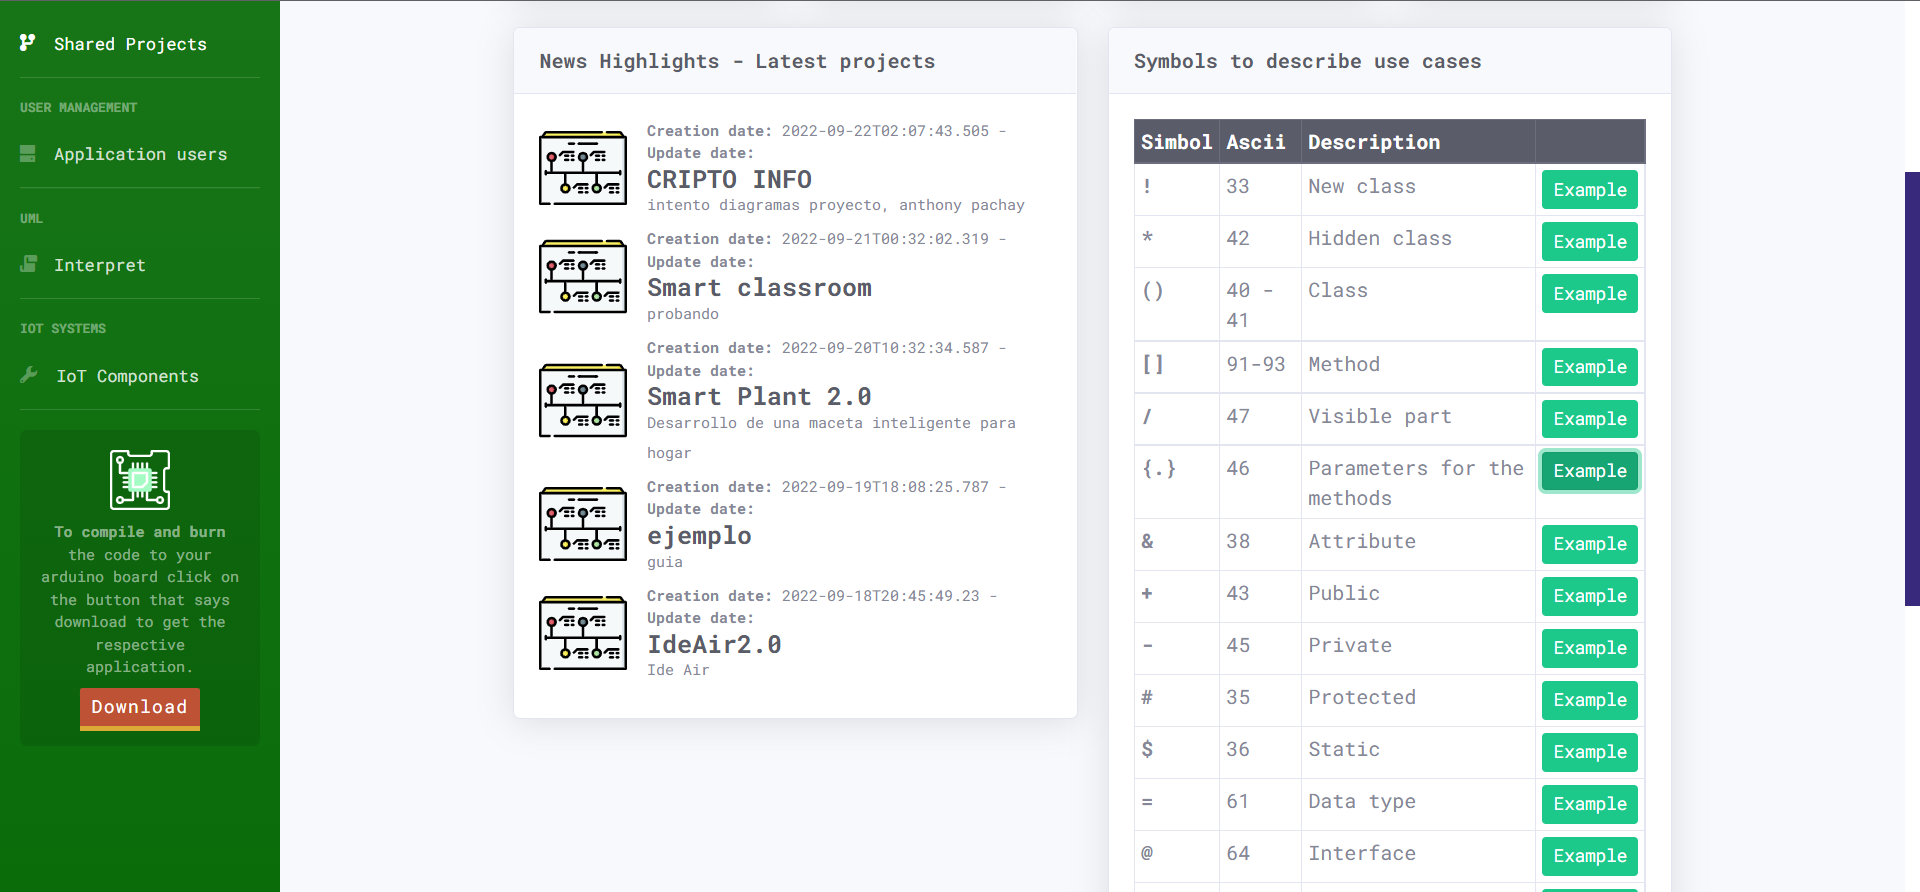
\includegraphics[width=14cm]{img/res_001.png}
	\label{fig:simbolostdd}
	\textbf{\\ FUENTE: PROPIA \\ ELABORADO: DÚVAL CARVAJAL SUÁREZ}
\end{figure}

En la lista de símbolos que se visualizar en la figura anterior se encuentra un botón que dice \textit{"Example"}. Si presionamos en ese botón se pudo observar un ejemplo detallado sobre como se deben utilizar los símbolos para tratar de especificar algún objeto del diagrama de clases que se generar mediante la descripción del caso de uso pertinente (ver figuras \ref{fig:ejemploclase}, \ref{fig:ejemploparametro}).

\begin{figure}[H]
	\caption{Ejemplo de como se debe utilizar el símbolo respectivo para crear una clase.}
	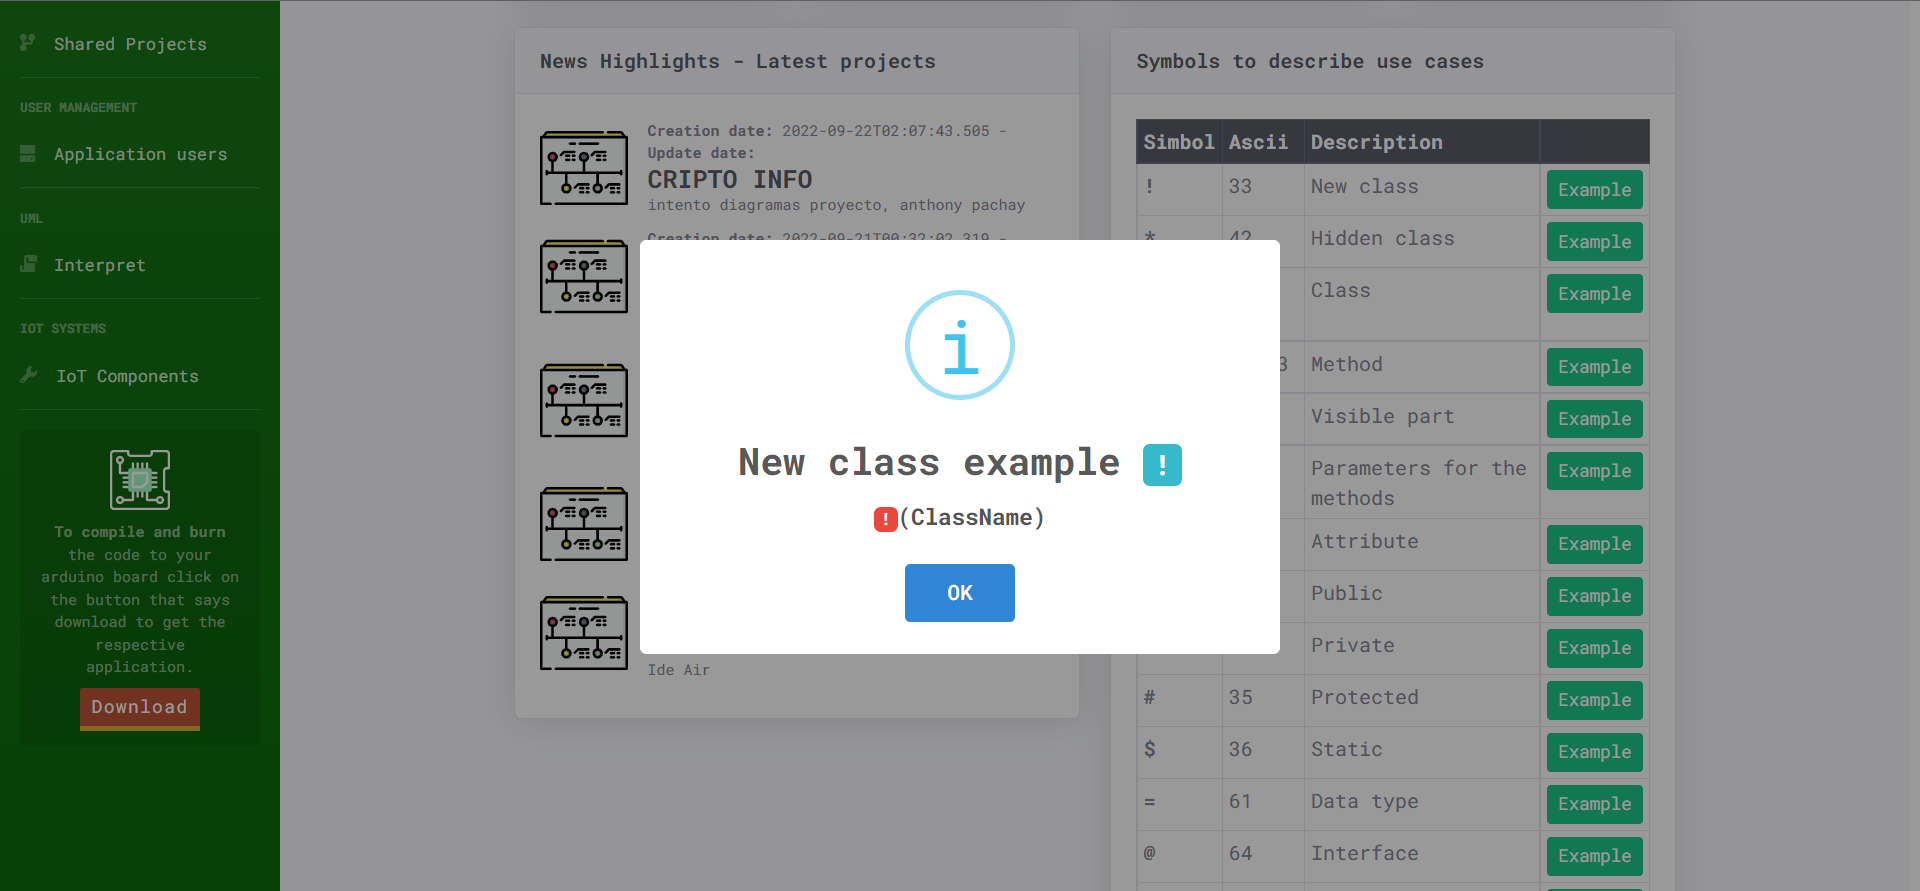
\includegraphics[width=14cm]{img/res_002.png}
	\label{fig:ejemploclase}
	\textbf{\\ FUENTE: PROPIA \\ ELABORADO: DÚVAL CARVAJAL SUÁREZ}
\end{figure}

\begin{figure}[H]
	\caption{Ejemplo de como se debe utilizar el símbolo respectivo generar los parámetros de un método declarado con el lenguaje de símbolos.}
	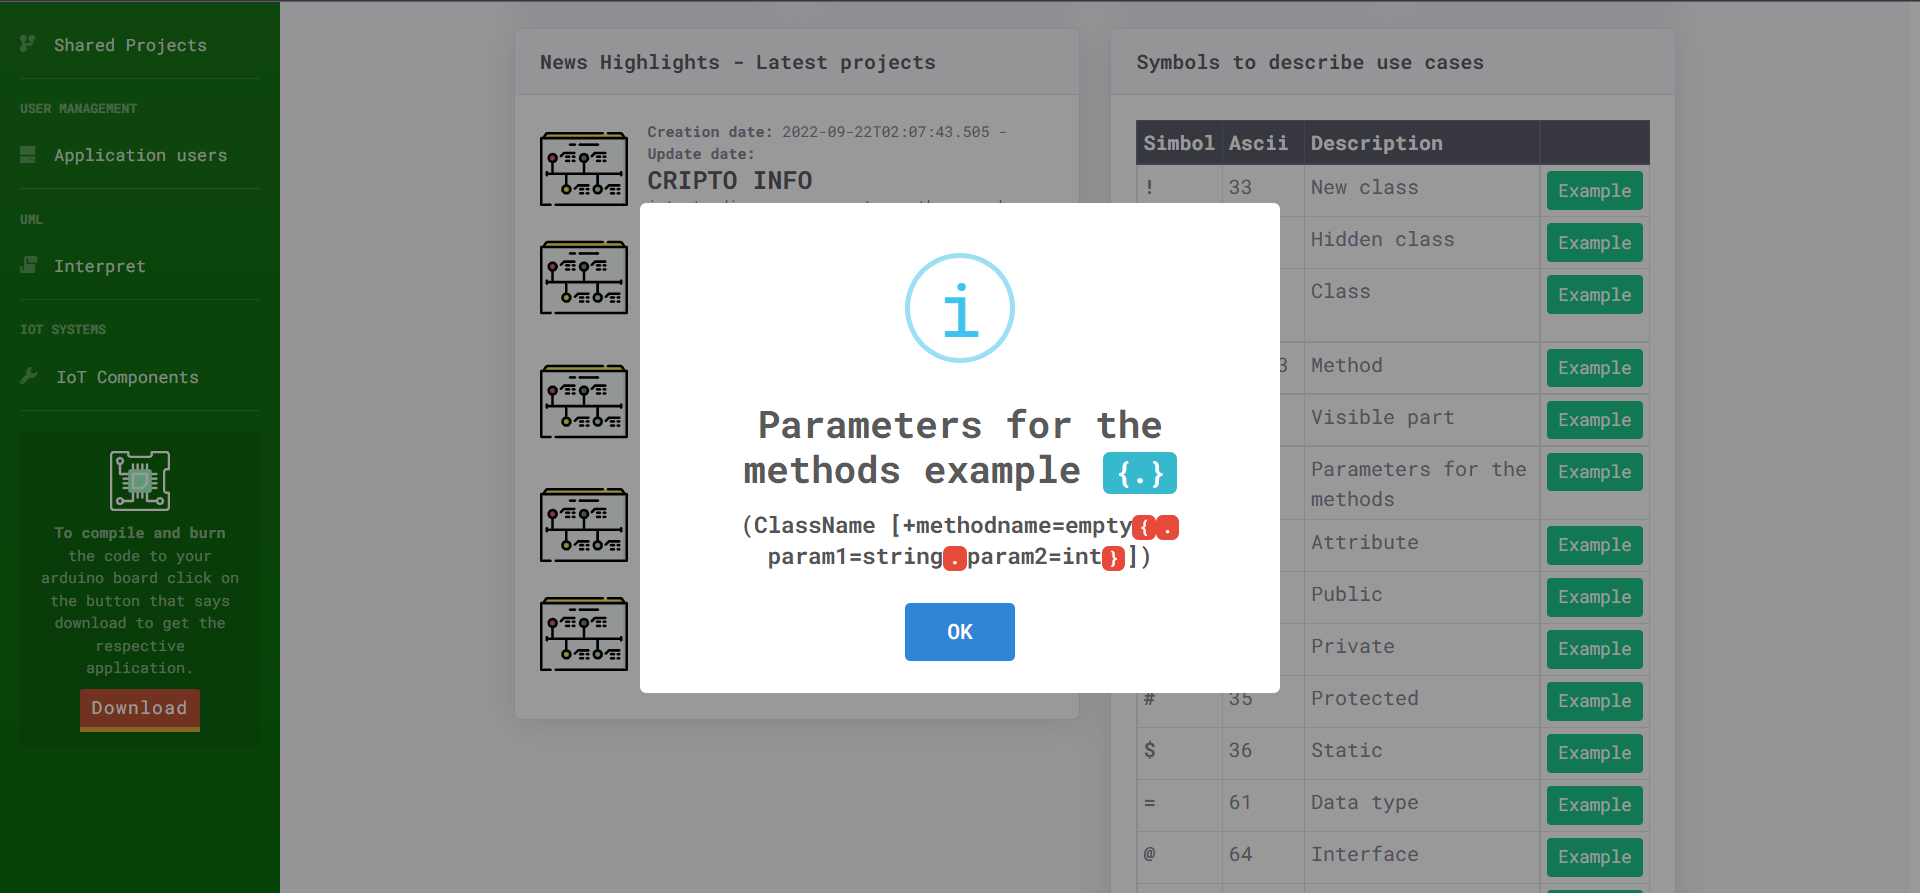
\includegraphics[width=14cm]{img/res_003.png}
	\label{fig:ejemploparametro}
	\textbf{\\ FUENTE: PROPIA \\ ELABORADO: DÚVAL CARVAJAL SUÁREZ}
\end{figure}

Luego de tener una idea general sobre los símbolos que utiliza la herramienta se especificaron detalladamente los significados de cada símbolo y como puede ser utilizado en las descripciones de los casos de uso.  

\begin{itemize}
	\item \textbf{Asterisco *}: Este símbolo sirve para ocultar cualquier carácter que se encuentre redactado después el. Esto permitirá al momento de interpretar la descripción del caso de uso ingresada eliminar los caracteres mezclados con los símbolos y solo dejar visibles los caracteres normales formando un texto natural que pueda ser entendido por cualquier persona regular. \textbf{Ejemplo:}
	
	\begin{verbatim}
		* texto de prueba
	\end{verbatim}
	
	\item \textbf{Paréntesis de apertura y cierre ()} : Este símbolo sirve para especificar uno de los componentes más importantes del diagrama de clases, dentro de los paréntesis de apertura y cierra se deberá especificar el nombre de la clase u objeto que se pretende generar de forma automática. Cabe mencionar que, si se escribe el nombre de clase separada por espacios, la librería deberá omitir estos espacios y auto completarlos con la segunda letra después del espacio con mayúscula. \textbf{Ejemplo:}  
	
	\begin{verbatim}
		(Nombre de la clase)
	\end{verbatim}
	
	\item \textbf{Corchete de apertura y cierre []:} Este símbolo podrá ser utilizado dentro de los símbolos para crear las clases, permitirá definir Los métodos o funciones que pertenecerá a la clase respectiva. \textbf{Ejemplo:} 
	
	\begin{verbatim}
		(Nombre de la clase [+nombre del metodo=empty])
	\end{verbatim} 
	
	\item \textbf{Slash /:} Este símbolo es bastante interesante, con el se debe visualizar cualquier caracteres que se encuentre encerrado de un slash de apertura y otro slash de cierre. Este símbolo se lo deberá usar cuando todos los caracteres se encuentren después del símbolo del asterisco, la idea es permitir que se visualicen caracteres específicos dentro de los datos técnicos para generar el diagrama de clases, sin afectar el uso de los demás símbolos. \textbf{Ejemplo:}
	
	\begin{verbatim}
		(Nombre de la clase &+/nombre/=string)
	\end{verbatim} 
	
	\item \textbf{Llaves de apertura y llaves de cierre con punto \{.\}:} Con el símbolo de las llaves se podrá definir los parámetros de entrada para los métodos o funciones de las clases. Cada parámetro estará separado por un punto, además se deberá utilizar el símbolo del igual (=) para especificar su tipo de dato. Cada recalcar que todos los atributos también deberán estar especificados dentro de las llaves de apertura y cierre. \textbf{Ejemplo:}
	
	\begin{verbatim}
		(Nombre de la clase [+nombre del metodo=empty
		{.param1=string.param2=strgin}])
	\end{verbatim}
	
	\item \textbf{Ampersand \&: } Este símbolo debe permitir declarar los atributos de la clase que fue creada con el símbolo anterior. Existen otros símbolos que interviene en la creación de otros componentes del diagrama de clases, más adelante se detallaran para que sirven. \textbf{Ejemplo:}
	
	\begin{verbatim}
		(Nombre de la clase &+atributo uno=string &+atributo 
		dos=string)
	\end{verbatim}
	
	\item \textbf{Visibilidad +: } El símbolo de suma permite especificar que la visibilidad del atributo, método o función será de manera pública. \textbf{Ejemplo:}
	
	En este ejemplo se visualiza la forma en cómo utilizar el símbolo de suma en atributos de clase.
	
	\begin{verbatim}
		(Nombre de la clase &+atributo uno=string &+atributo 
		dos=string)
	\end{verbatim}
	
	En este ejemplo se visualiza la forma en cómo utilizar el símbolo de suma en métodos o funciones de clase.
	
	\begin{verbatim}
		(Nombre de la clase [+nombre del metodo=empty
		{.param1=string.param2=strgin}])
	\end{verbatim}
	
	\item \textbf{Visibilidad -: } El símbolo de resta permite especificar que la visibilidad del atributo, método o función será de manera privada. \textbf{Ejemplo:}
	
	En este ejemplo se visualiza la forma en cómo utilizar el símbolo de suma en atributos de clase.
	
	\begin{verbatim}
		(Nombre de la clase &-atributo uno=string &-atributo 
		dos=string)
	\end{verbatim}
	
	En este ejemplo se visualiza la forma en cómo utilizar el símbolo de suma en métodos o funciones de clase.
	
	\begin{verbatim}
		(Nombre de la clase [-nombre del metodo=empty
		{.param1=string.param2=strgin}])
	\end{verbatim}
	
	\item \textbf{Visibilidad \#: } El símbolo de almohadilla permite especificar que la visibilidad del atributo, método o función será de manera protegida. \textbf{Ejemplo:}
	
	En este ejemplo se visualiza la forma en cómo utilizar el símbolo de suma en atributos de clase.
	
	\begin{verbatim}
		(Nombre de la clase &#atributo uno=string &#atributo 
		dos=string)
	\end{verbatim}
	
	En este ejemplo se visualiza la forma en cómo utilizar el símbolo de suma en métodos o funciones de clase.
	
	\begin{verbatim}
		(Nombre de la clase [#nombre del metodo=empty
		{.param1=string.param2=strgin}])
	\end{verbatim}
	
	\item \textbf{Visibilidad \$: } El símbolo de dólar permite especificar que la visibilidad del atributo, método o función será de manera estática. \textbf{Ejemplo:}
	
	En este ejemplo se visualiza la forma en cómo utilizar el símbolo de suma en atributos de clase.
	
	\begin{verbatim}
		(Nombre de la clase &$atributo uno=string &$atributo 
		dos=string)
	\end{verbatim}
	
	En este ejemplo se visualiza la forma en cómo utilizar el símbolo de suma en métodos o funciones de clase.
	
	\begin{verbatim}
		(Nombre de la clase [$nombre del metodo=empty
		{.param1=string.param2=strgin}])
	\end{verbatim}
	
	\item \textbf{Igual =:} El símbolo de igual debe permitir asignar el tipo de dato a los atributos, métodos o funciones declaradas dentro de la clase. En el caso de los métodos de tipo \textbf{void}  se deberá utilizar la palabra \textit{empty} indiciando que es un método que retornara ningún valor. \textbf{Ejemplo:}
	
	\begin{verbatim}
		{.param1=string.param2=strging}
	\end{verbatim}
	
	\item \textbf{Arroba @:} El símbolo de arroba se lo utiliza dentro de los paréntesis que permiten generar una clase del diagrama. Pero se recuerda que en el diagrama de clases también se pueden crear interfaces. El objetivo de este simbolo es utilizarlo dentro de los paréntesis pero el interprete identifica que sera una interfaz la que se deberá crear. \textbf{Ejemplo:}
	  
	\begin{verbatim}
		(@nombre interfaz)
	\end{verbatim}

	\item  \textbf{Signo de interrogación apertura y cierre ¿?:} El simbolo de interrogación se lo utiliza para generar otro tipo de objeto principal del diagrama de clases. El objetivo principal de este simbolo es generar los enum. \textbf{Ejemplo:}
	
	\begin{verbatim}
		¿enumTest?
	\end{verbatim}

	\item \textbf{Cierra comillas bajas »:} El simbolo de cierre comillas bajas se lo utiliza para agregar atributos a un objeto principal del diagrama de clases. El objetivo principal de este simbolo es atributos dentro de los objetos enum. \textbf{Ejemplo:}
	
	\begin{verbatim}
		¿enumTest »atributoUno »atributoDos?
	\end{verbatim}

	\item \textbf{Porcentaje \%:} El simbolo de porcentaje sirve para agregar nuevos constructores a las clases que ya fueron definidas, ademas para especificar sus parámetros se utiliza los mismos símbolos para agregara atributos a la clase, con la diferencia que los parámetros van separados por la coma. \textbf{Ejemplo:}
	
	\begin{verbatim}
		*(class %.class=Class, .param=string%)
	\end{verbatim}
	  
\end{itemize}

Dentro del diagrama de clases existen diferentes tipos de relaciones con las que se pueden relacionar las clases que se encuentran definidas. Para implementar las relaciones también se utilizan una combinación de símbolos que permitan detectarlas y la librería se encarga de generarlas. A continuación se especificaran los símbolos que se utilizan para los tipos de relaciones en el diagrama de clases:

\begin{itemize}
	\item \textbf{Simbolo de admiración de apertura ¡!:} Para indicar que se va realizar una relación entre 2 objetos del diagrama de clases, el texto debe estar entre este simbolo tanto en su apertura y cierre.
	
	\item \textbf{Corchete de apertura y cierre []:} Dentro del simbolo de admiración se podrá indicar un texto como leyenda sobre la linea de la relación, esto indicara alguna palabra clave sobre la relación entre los objetos.
	
	\item \textbf{Cardinalidad 1 o n:} Sobre la linea de la relación se puede indicar una cardinalidad de uno a muchos. El numero \textit{\underline{1}} indicara que la cardinalidad es de 1 y si usa la letra \textit{\underline{n}} indicara que la cardinalidad des de muchos. Se los debe utilizar en la parte exterior de los corchetes.
	
	\item \textbf{Agregación > >:} Para indicar que el tipo de relación entre dos objetos del diagrama de clases se utiliza los símbolos de \textit{> >}. Se deben colocar en la parte exterior donde se el texto de cardinalidad. \textbf{Ejemplo:}
	
	\begin{verbatim}
		*¡claseUno 1>[texto de cardinalidad]>n claseDos!
	\end{verbatim}

	\item \textbf{Dependencia < <:} Para indicar que el tipo de relación entre dos objetos del diagrama de clases se utiliza los símbolos de \textit{< <}. Se deben colocar en la parte exterior donde se el texto de cardinalidad. \textbf{Ejemplo:}
	
	\begin{verbatim}
		*¡claseUno 1<[texto de cardinalidad]<n claseDos!
	\end{verbatim}

	\item \textbf{Generalización < >:} Para indicar que el tipo de relación entre dos objetos del diagrama de clases se utiliza los símbolos de \textit{<>}. Se deben colocar en la parte exterior donde se el texto de cardinalidad. \textbf{Ejemplo:}
	
	\begin{verbatim}
		*¡claseUno 1<[texto de cardinalidad]>n claseDos!
	\end{verbatim}

	\item \textbf{Asociación > <:} Para indicar que el tipo de relación entre dos objetos del diagrama de clases se utiliza los símbolos de \textit{> <}. Se deben colocar en la parte exterior donde se el texto de cardinalidad. \textbf{Ejemplo:}
	
	\begin{verbatim}
		*¡claseUno 1>[texto de cardinalidad]<n claseDos!
	\end{verbatim}
	
\end{itemize}

En la tabla se describe el código ASCII para escribir los símbolos mediante el teclado de una computadora. Se pretendió que cada simbolo tenga una combinación ASCII para que el analista pueda escribir cada simbolo con el teclado y no obtenerlo de alguna forma que sea complicada.

\begin{table}[h!]
	\caption{Código ASCII para cada simbolo del lenguaje.}
	\begin{tabular}{p{2cm}p{4cm}p{5cm}}
		\toprule
		\textbf{Simbolo} & \textbf{ASCII} & \textbf{Descripción} \\
		\midrule
		* & 33 & Ocultar texto \\
		\addlinespace
		( ) & 40 - 41 & Crear clase \\
		\addlinespace
		\textbf{[ ]} & 91 - 93 & Crear método \\
		\addlinespace
		/ & 47 & Parte visible \\
		\addlinespace
		\{.\} & 123 - 125	 & Parámetro de los métodos \\
		\addlinespace 	
		\& & 38 & Atributo de clase \\
		\addlinespace
		+ & 43 & Publico \\
		\addlinespace
		- & 45 & Privado \\
		\addlinespace
		\# & 35 & Protegido \\
		\addlinespace
		\$ & 36 & Estático \\
		\addlinespace
		= & 61 & Tipo de dato \\
		\addlinespace
		@ & 64 & Interfaz \\
		\addlinespace
		¿? & 168 - 63 & Enum \\
		\addlinespace
		\% & 37 & Constructores \\
		\addlinespace
		\bottomrule
	\end{tabular}
	\textbf{ \\ ELABORADO: DÚVAL CARVAJAL SUÁREZ}
\end{table}

Para definir los diferentes tipos de relaciones que se usaran en el diagrama de clases. En la tabla se visualiza un grupo de símbolos que servirán para crear las relaciones de tipo: agregación, dependencia, herencia o generalización y asociación. 

\begin{table}[h!]
	\caption{Código ASCII para cada simbolo del lenguaje que especifican las relaciones.}
	\begin{tabular}{p{2cm}p{4cm}p{6cm}}
		\toprule
		\textbf{Simbolo} & \textbf{ASCII} & \textbf{Descripción} \\
		\midrule
		!¡ & 33 - 173 & Crear relación \\
		\addlinespace
		\textbf{[ ]} & 91 - 93 & Especificar leyenda en la relación \\
		\addlinespace
		1[ ]1 & -- & Cardinalidad de uno a uno \\
		\addlinespace
		1[ ]n & -- & Cardinalidad de uno a muchos \\
		\addlinespace
		n[ ]1 & -- & Cardinalidad de muchos a uno \\
		\addlinespace
		> > & 62 - 62 & Agregación \\
		\addlinespace
		< < & 60 - 60 & Dependencia \\
		\addlinespace
		< > & 60 - 62 & Generalización \\
		\addlinespace
		> < & 62 - 60 & Asociación \\
		\addlinespace
		\bottomrule
	\end{tabular}
	\textbf{ \\ ELABORADO: DÚVAL CARVAJAL SUÁREZ}
\end{table}

Luego de a ver recopilado todos los símbolos que la librería va interpretar, el docente proporciono 1 caso de uso. Ademas proporciono el gráfico del diagrama de clases que se escribió en los casos de uso. En la figura \ref{fig:usecasetest} se observa el caso de uso de prueba para saber que objetos debe generar la librería.

\begin{figure}[h!]
	\caption{Diagrama de casos de uso para las pruebas.}
	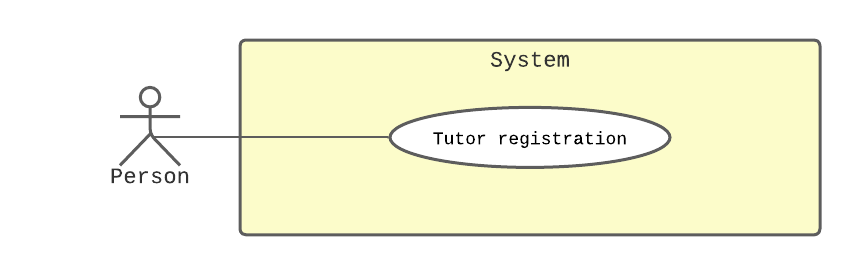
\includegraphics[width=15cm]{img/usecaseTest.png}
	\label{fig:usecasetest}
	\textbf{\\ ELABORADO: DÚVAL CARVAJAL SUÁREZ}
\end{figure}

Para comprender totalmente las acciones que se deben ejecutar en le caso de uso que se usara como prueba, esta escrito en 2 distintas formas. En la tabla \ref{tab:usecasetutorregistration} se observa la descripción del caso de uso en lenguaje natural especificando todas las acciones con el objetivo que cualquier persona regular logre entender. En la tabla \ref{tab:usecasetutorregistration_symbol} se observa la misma descripción del caso de uso pero utilizando los símbolos.

\newpage  

\begin{table}[h!]
	\caption{Descripción del caso de uso para Tutor registration.}
	\label{tab:usecasetutorregistration}
	\begin{tabular}{| p{3cm} | p{11cm} |}
		\hline
		\textbf{Use case:} & Tutor registration \\ \hline
		\textbf{Actors:} & Person \\ \hline
		\textbf{Postcondition:} & User registered in the database. \\ \hline
		\textbf{Precondition:} & The user exists in the database. \\ \hline
		\textbf{Purpose:} & Ingresar a la interfaz principal de la aplicación \\ \hline
		\textbf{Abstract:} & 
		Permite identificar las credenciales del usuario que intenta ingresar al sistema, de esa forma verificar el tipo de usuario que ingresa. \\ \hline
		\textbf{Type:} & Primary \\ \hline
		\multicolumn{2}{ |c| }{\textbf{Normal flow}} \\ \hline
	\end{tabular}
	\begin{tabular}{| p{7cm} | p{7cm} |}
		1. This use case starts when a person wants to register as a tutor user in the system.  & \\ \hline
		2. The person accesses then User Registration interface. & \\ \hline
		& 3. Shows you the fields to fill in the interface user registration : first name last name date of birth gender phone number email username password. It should be taken into account that the registration of a Person has a User. There are states that can be Disabled o Enabled that each User will have a Status . There are also several types of users, which are Tutor or Patient or Admin and every User will have a UserType. In addition, the system assigns an id when storing it. \\ \hline
		4. The person enters all the data required by the view, and clicks submit. & \\ \hline
		& 5. Create a person object. \\ \hline
		& 6. Create a tutor object. \\ \hline
		& 7. Create an user object. \\ \hline
		& 8. Saves the tutor data in the database. \\ \hline
		& 9. Saves the user data in the database. \\ \hline
		& 10. This use case ends when the system displays the login Interface.  \\ \hline
	\end{tabular} \\
	\textbf{ \\ ELABORADO: DÚVAL CARVAJAL SUÁREZ}
\end{table}

Para la elaboración de la descripción del caso de uso con los símbolos proporcionaron información de un diagrama de clases que ya se encontraba realizado. El objetivo de este caso de uso era escribir todas las acciones con información técnica que permita crear el diagrama de clases lo mas parecido posible al original. En la figura \ref{fig:cdtest} se observa el diagrama de clases creado de forma manual.

\begin{figure}[h!]
	\caption{Diagrama de clases de prueba}
	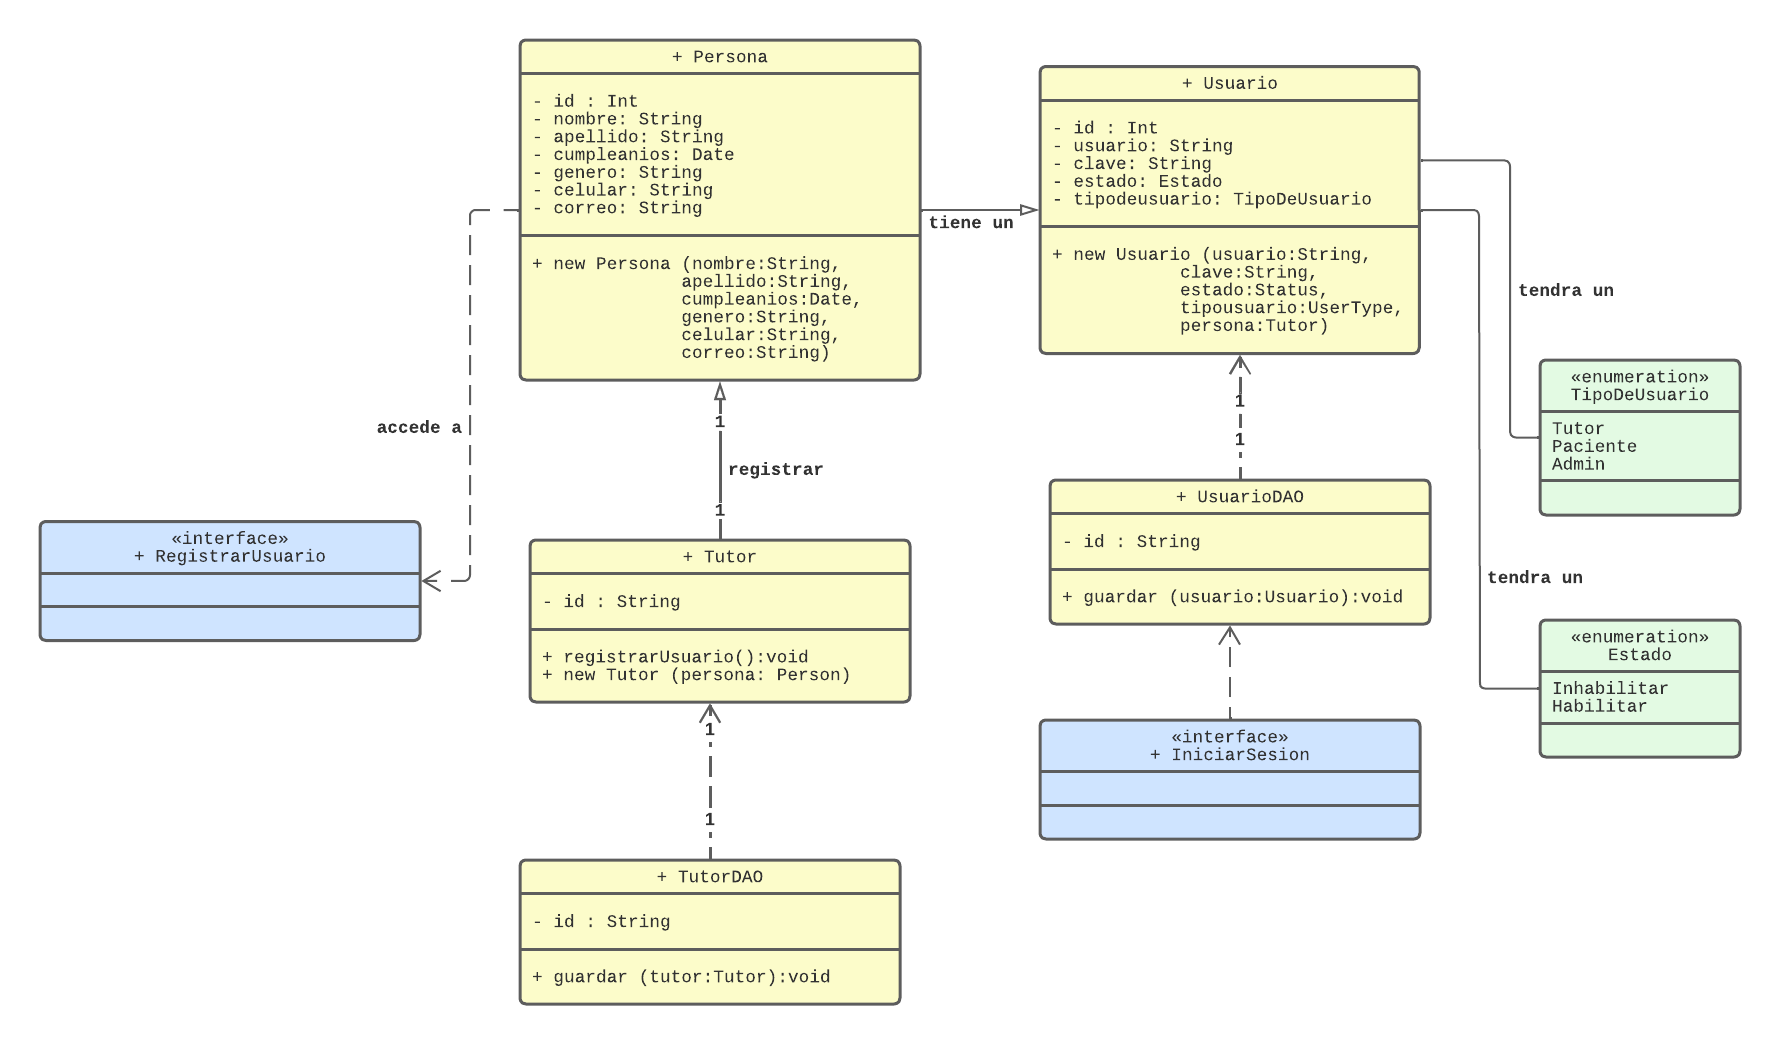
\includegraphics[width=15.5cm]{img/cdtest.png}
	\label{fig:cdtest}
	\textbf{\\ ELABORADO: DÚVAL CARVAJAL SUÁREZ}
\end{figure}

\begin{table}[h!]
	\caption{Descripción del caso de uso para Tutor registration.}
	\label{tab:usecasetutorregistration_symbol}
	\begin{tabular}{| p{3cm} | p{11cm} |}
		\hline
		\textbf{Use case:} & Tutor registration \\ \hline
		\textbf{Actors:} & Person \\ \hline
		\textbf{Postcondition:} & User registered in the database. \\ \hline
		\textbf{Precondition:} & The user exists in the database. \\ \hline
		\textbf{Purpose:} & Ingresar a la interfaz principal de la aplicación \\ \hline
		\textbf{Abstract:} & 
		Permite identificar las credenciales del usuario que intenta ingresar al sistema, de esa forma verificar el tipo de usuario que ingresa. \\ \hline
		\textbf{Type:} & Primary \\ \hline
		\multicolumn{2}{ |c| }{\textbf{Normal flow}} \\ \hline
	\end{tabular}
	\begin{tabular}{| p{7cm} | p{7cm} |}
		1. This use case starts when a person *(person \&-id=int) wants to register as a tutor *(tutor \&-id=int [+userRegistration=Tutor]) user in the system. *¡tutor 1<[register]>n Person! & \\ \hline
		2. The person accesses then User Registration *(@User Registration) interface. *¡person1<[accesses]<1 User Registration! & \\ \hline

	\end{tabular}
\end{table}

\begin{table}[]
	\begin{tabular}{| p{7cm} | p{7cm} |}
		\hline
		& 3. Shows you the fields to fill in the interface user registration *(@User registration): *(Person \&-/first name/=String, \&-/last name/=String, \&-/date of birth/=Date, \&-/gender/=String, \&-/phone number/=String, \&-/email/=String) *(User \&-id=Int, \&-/username/=String, \&-/password/=String \&-status=Status \&-user type=UserType). It should be taken into account that the registration of a *!/Person/ u<[/has a/]>u /User/¡. There are states that can be *¿Status »/Disabled/ /o/ »/Enabled/? that each *¡/User/ u>[/will have a/]<u /Status/! . There are also several types of users, which are *¿UserType »/Tutor/ /or/ »/Patient/ /or/ »/Admin/? and every *¡/User/ u>[/will have a/]<u /UserType/!. In addition, the system assigns an id when storing it. \\ \hline
		4. The person enters all the data required by the view, and clicks submit. & \\ \hline
		& 5. Create a *(/person/ \%.first name=String, .last name=String, .date of birth=Date, .gender=String, .phone number=String, .email=String\%) object. \\ \hline
		& 6. Create a *(/tuto/r \%.person=Person\%) object \\ \hline
		& 7. Create an *(/user/ \%.username=String, .password=String, .status=Status, .user type=UserType, .person=Tutor\%) object \\ \hline
		& 8. *(TutorDAO \&id=Int [/Save/=Tutor{.tutor=Tutor}])s the tutor data in the database. *¡TutorDAO<[]< tutor!. \\ \hline
		& 9. *(UserDAO \&-id=Int [/Save/=User{.user=User}])s the user data in the database. *¡UserDAO <[]< User!. \\ \hline
		& 10. This use case ends when the system displays the *(@Login) login Interface. *¡Login u<[]<u UserDAO! \\ \hline
	\end{tabular} \\
\textbf{\\ ELABORADO: DÚVAL CARVAJAL SUÁREZ}
\end{table}

\section{Modelamiento}

Se utilizo el lenguaje de programación JavaScript con la intención de generar un paquete totalmente exportable a otros proyectos que requieran utilizar la librería para generar sus propios diagramas con otras librerías de dibujo. Para empezar con el diseño o modelamiento de la librería se especificó el proceso normal que deberá seguir la al momento de recibir como datos de entrada las descripciones de los casos de uso. En la figura \ref{fig:armadillocasodeuso} se observa el proceso que se llevara a cabo de forma general la ejecución de la librería.

En la figura \ref{fig:armadillocasodeuso} se pude observar el diagrama de casos de uso que explica las acciones que el analista podrá realizar al momento de implementar la librería, o podrá utilizar la aplicación de demostración


\begin{figure}[h!]
	\caption{Diagrama de casos de uso armadillo.}
	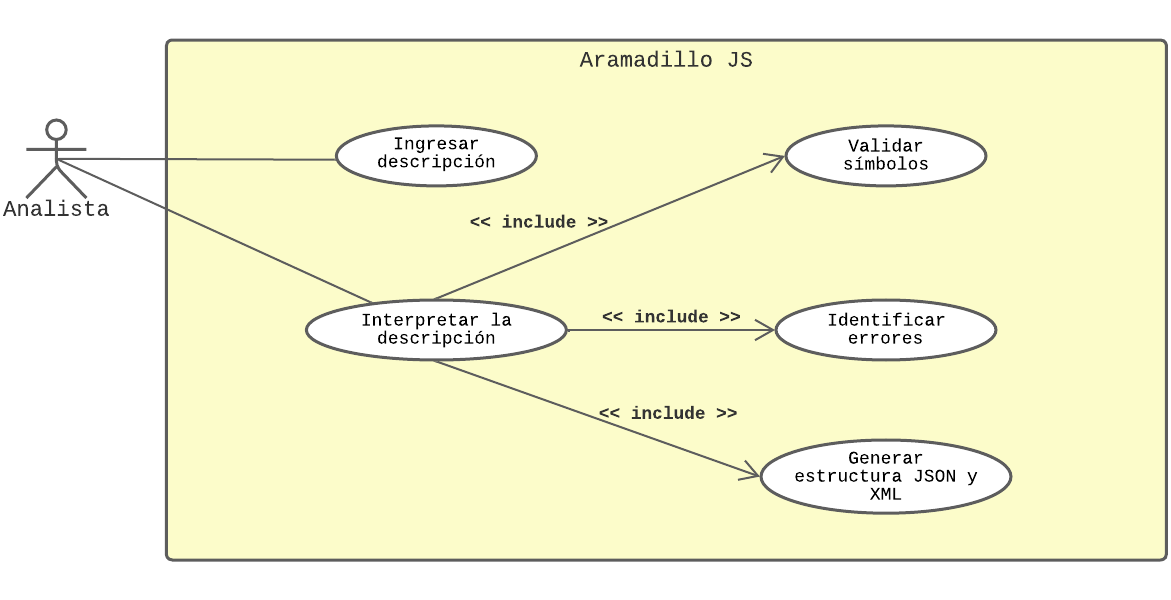
\includegraphics[width=15cm]{img/modelamientocasodeuso.png}
	\label{fig:armadillocasodeuso}
	\textbf{\\ \\ ELABORADO: DÚVAL CARVAJAL SUÁREZ}
\end{figure} 

A continuación, se detallarán las descripciones de los casos de uso que se observan en la imagen anterior. Se especificaran todos los pasos que la librería debe recibir para responder de forma correcta. Se recuerda que la librería no cuenta con acceso a datos o algún tipo de información en la nube.  

En la tabla \ref{tab:ucingresardescripcion} se detallan los pasos que se siguen al momento de ingresar las descripciones de los casos de uso que se pretenden interpretar.

\newpage

\begin{table}[H]
	\caption{Descripción del caso de uso para ingresar la descripción.}
	\label{tab:ucingresardescripcion}
	\begin{tabular}{| p{3cm} | p{11cm} |}
		\hline
		\textbf{Caso de uso:} & Ingresar descripción \\ \hline
		\textbf{Actores:} & Analista \\ \hline
		\textbf{Precondición:} & Tener instanciada la librería en su proyecto web, o debe utilizar la aplicación de demostración. \\ \hline
		\textbf{Postcondición:} & Descripción ingresada en la librería. \\ \hline
		\textbf{Propósito:} & Ingresar un párrafo de la descripción del caso de uso. \\ \hline
		\textbf{Resumen:} & Permite ingresar un párrafo de toda la descripción del caso de uso utilizando el lenguaje de símbolos. \\ \hline
		\textbf{Tipo:} & Primario \\ \hline
		\multicolumn{2}{ |c| }{\textbf{Flujo normal}} \\ \hline
	\end{tabular}
	\begin{tabular}{| p{7cm} | p{7cm} |}
		1. Este caso de uso inicia el analista pretende ingresar la descripción del caso de uso. & \\ \hline
		2. Redacta la descripción del caso uso utilizando el lenguaje de símbolos.  & \\ \hline
		& 3. Muestra la caja de texto donde se debe colocar la descripción del caso de uso con el lenguaje de símbolos. \\ \hline
		4. Este caso de uso finaliza cuando el analista ingresa la descripción del caso de uso. & \\ \hline		
		\multicolumn{2}{ |c| }{\textbf{Flujos alternos}} \\ \hline
	\end{tabular}
	\begin{tabular}{| p{7cm} | p{7cm} |}
		
	\end{tabular} \\
	\textbf{ \\ ELABORADO: DÚVAL CARVAJAL SUÁREZ}
\end{table}

\newpage

\begin{table}[h!]
	\caption{Descripción del caso de uso para interpretar la descripción.}
	\label{tab:ucinterpretardescripcion}
	\begin{tabular}{| p{3cm} | p{11cm} |}
		\hline
		\textbf{Caso de uso:} & Interpretar descripción \\ \hline
		\textbf{Actores:} & Analista \\ \hline
		\textbf{Precondición:} & Tener ingresada la descripción a interpretar redactada con el lenguaje de símbolos. \\ \hline
		\textbf{Postcondición:} & Obtener la descripción redactada en lenguaje natural. \\ \hline
		\textbf{Propósito:} & Obtener la descripción del caso de uso e interpretar los símbolos del lenguaje. \\ \hline
		\textbf{Resumen:} & Permite identificar cada simbolo del lenguaje para identificar los objetos que se deben crear en el diagrama de clases. \\ \hline
		\textbf{Tipo:} & Primario \\ \hline
		\multicolumn{2}{ |c| }{\textbf{Flujo normal}} \\ \hline
	\end{tabular}
	\begin{tabular}{| p{7cm} | p{7cm} |}
		\textbf{Acción del actor} & \textbf{Respuesta del sistema} \\ \hline	
		1. Este caso de uso inicia cuando el analista pretende interpretar la descripción del caso de uso. & \\ \hline		
		2. El analista da la orden de interpretar la descripción con el lenguaje de símbolos. & \\ \hline
		& 3. Muestra dentro de un apartado denominado consola, todos los procesos que realizaron al momento de interpretar la descripción. Ademas de mostrar rápidamente el texto redactado en lenguaje normal. \\ \hline
		4. El analista se dirige a la pestaña de "Class diagram".  & \\ \hline
		& 5. Muestra el grafico del diagrama de clases generado por la librería. Se dibujan los objetos que pudieron ser identificados por los simbolos usados. \\ \hline
		6. El analista se dirige a la pestaña de "JSON". & \\ \hline
		& 7. Muestra la estructura JSON generada. \\ \hline
		8. El analista se dirige a la pestaña de "XML".  & \\ \hline
		& 9. Muestra la estructura XML generada. \\ \hline
		10. Este caso de uso finaliza cuando el analista descarga las estructuras JSON o XML para posteriores proyectos. & \\ \hline			
		\multicolumn{2}{ |c| }{\textbf{Flujos alternos}} \\ \hline
	\end{tabular}
	\begin{tabular}{| p{7cm} | p{7cm} |}
		
	\end{tabular} \\
	\textbf{ \\ ELABORADO: DÚVAL CARVAJAL SUÁREZ}
\end{table}

\begin{table}[H]
	\caption{Descripción del caso de uso para validar símbolos.}
	\label{tab:ucvalidarsimbolos}
	\begin{tabular}{| p{3cm} | p{11cm} |}
		\hline
		\textbf{Caso de uso:} & Validar símbolos \\ \hline
		\textbf{Actores:} & Analista \\ \hline
		\textbf{Precondición:} & La descripción del caso de uso debe contar con los símbolos del lenguaje. \\ \hline
		\textbf{Postcondición:} & Todos los símbolos serán omitidos en el texto que sea interpretado. \\ \hline
		\textbf{Propósito:} & Identificar los objetos para generar el diagrama de clases \\ \hline
		\textbf{Resumen:} & Permite identificar los símbolos que son usados para redactar los casos de uso. Ademas de verificar si se los esta usando de forma correcta. \\ \hline
		\textbf{Tipo:} & Secundario \\ \hline
		\multicolumn{2}{ |c| }{\textbf{Flujo normal}} \\ \hline
	\end{tabular}
	\begin{tabular}{| p{7cm} | p{7cm} |}
		& 1. Este caso de uso inicia cuando la descripción del caso fue ingresada con los símbolos del lenguaje. \\ \hline
		& 2. Se identifican los tipos de simbolos que tiene el lenguaje, si son simbolos con apertura y cierre o son individuales. \\ \hline
		& 3. Se verifica que los símbolos están usándose de forma correcta sin combinarlos con otros símbolos desconocidos.  \\ \hline
		& 4. Este caso de uso finaliza cuando se identificaron todos los símbolos de la descripción y oculta los símbolos para obtener un texto natural.  \\ \hline		
		\multicolumn{2}{ |c| }{\textbf{Flujos alternos}} \\ \hline
	\end{tabular}
	\begin{tabular}{| p{7cm} | p{7cm} |}
		
	\end{tabular} \\
	\textbf{ \\ ELABORADO: DÚVAL CARVAJAL SUÁREZ}
\end{table}

\begin{table}[H]
	\caption{Descripción del caso de uso para identificar errores.}
	\label{tab:ucidentificarerror}
	\begin{tabular}{| p{3cm} | p{11cm} |}
		\hline
		\textbf{Caso de uso:} & Identificar errores \\ \hline
		\textbf{Actores:} & Analista \\ \hline
		\textbf{Precondición:} & La descripción del caso de uso debe contar con los símbolos del lenguaje. \\ \hline
		\textbf{Postcondición:} & Todos los símbolos serán omitidos en el texto que sea interpretado. \\ \hline
		\textbf{Propósito:} & Permite identificar la mala escritura de las descripciones de los casos de uso. \\ \hline
		\textbf{Resumen:} & Identificar los posibles errores que se pueden cometer al momento de usar los símbolos en las descripciones de los casos de uso. \\ \hline
		\textbf{Tipo:} & Secundario \\ \hline
		\multicolumn{2}{ |c| }{\textbf{Flujo normal}} \\ \hline
	\end{tabular}
	\begin{tabular}{| p{7cm} | p{7cm} |}
		& 1. Este caso de uso inicia cuando la descripción del caso fue ingresada con los símbolos del lenguaje. \\ \hline
		& 2. Se identifican los tipos de simbolos que tiene el lenguaje, si son simbolos con apertura y cierre o son individuales. \\ \hline
		& 3. Si existen inconsistencias en la redacción de la descripción del caso de uso, se empieza acumular mensajes de alerta.   \\ \hline
		& 4.  Este caso de uso finaliza mostrando los mensajes en un apartado y clasificando los mensajes acumulados mediante un color diferentes: Azul para información, amarillo para advertencia, verde para exitoso y rojo para notificar errores graves. \\ \hline		
		\multicolumn{2}{ |c| }{\textbf{Flujos alternos}} \\ \hline
	\end{tabular}
	\begin{tabular}{| p{7cm} | p{7cm} |}
		
	\end{tabular} \\
	\textbf{ \\ ELABORADO: DÚVAL CARVAJAL SUÁREZ}
\end{table}

\begin{table}[H]
	\caption{Descripción del caso de uso para generar estructura json y xml.}
	\label{tab:ucgenerarjsonxml}
	\begin{tabular}{| p{3cm} | p{11cm} |}
		\hline
		\textbf{Caso de uso:} & Generar estructura JSON y XML \\ \hline
		\textbf{Actores:} & Analista \\ \hline
		\textbf{Precondición:} & La descripción del caso de uso debe contar con los símbolos del lenguaje. \\ \hline
		\textbf{Postcondición:} & Todos los símbolos serán omitidos en el texto que sea interpretado. \\ \hline
		\textbf{Propósito:} & Generar 2 estructuras con la información necesaria del diagrama de clases. \\ \hline
		\textbf{Resumen:} & Permite obtener toda la estructura del diagrama de clases generado en formato JSON Y XML \\ \hline
		\textbf{Tipo:} & Secundario \\ \hline
		\multicolumn{2}{ |c| }{\textbf{Flujo normal}} \\ \hline
	\end{tabular}
	\begin{tabular}{| p{7cm} | p{7cm} |}
		& 1. Este caso de uso inicia cuando la descripción del caso fue ingresada con los símbolos del lenguaje. \\ \hline
		& 2. Buscar los objetos que fueron identificados por los símbolos e ir armando el json y xml. \\ \hline
		& 3. Este caso de uso finaliza cuando se muestra por completo el json y xml uniendo todos los objetos del diagrama de clases  \\ \hline		
		\multicolumn{2}{ |c| }{\textbf{Flujos alternos}} \\ \hline
	\end{tabular}
	\begin{tabular}{| p{7cm} | p{7cm} |}
		
	\end{tabular} \\
	\textbf{ \\ ELABORADO: DÚVAL CARVAJAL SUÁREZ}
\end{table}

Para cumplir con los requisitos recopilados en la fase anterior se realizaron diagramas de flujo para realizar el análisis pertinente a lo que la librería debe cumplir. Esto permitirá identificar las posibles fallas que se mostrarían al momento de estar utilizando la librería. En la figura \ref{fig:algoritmoerror} se observa el algoritmo que permitió identificar los errores en la escritura de las descripciones de los casos de uso utilizando el lenguaje de símbolos.

\begin{figure}[h!]
	\caption{Diagrama de flujo para detectar errores en las descripciones de los casos de uso utilizando un el lenguaje de símbolos.}
	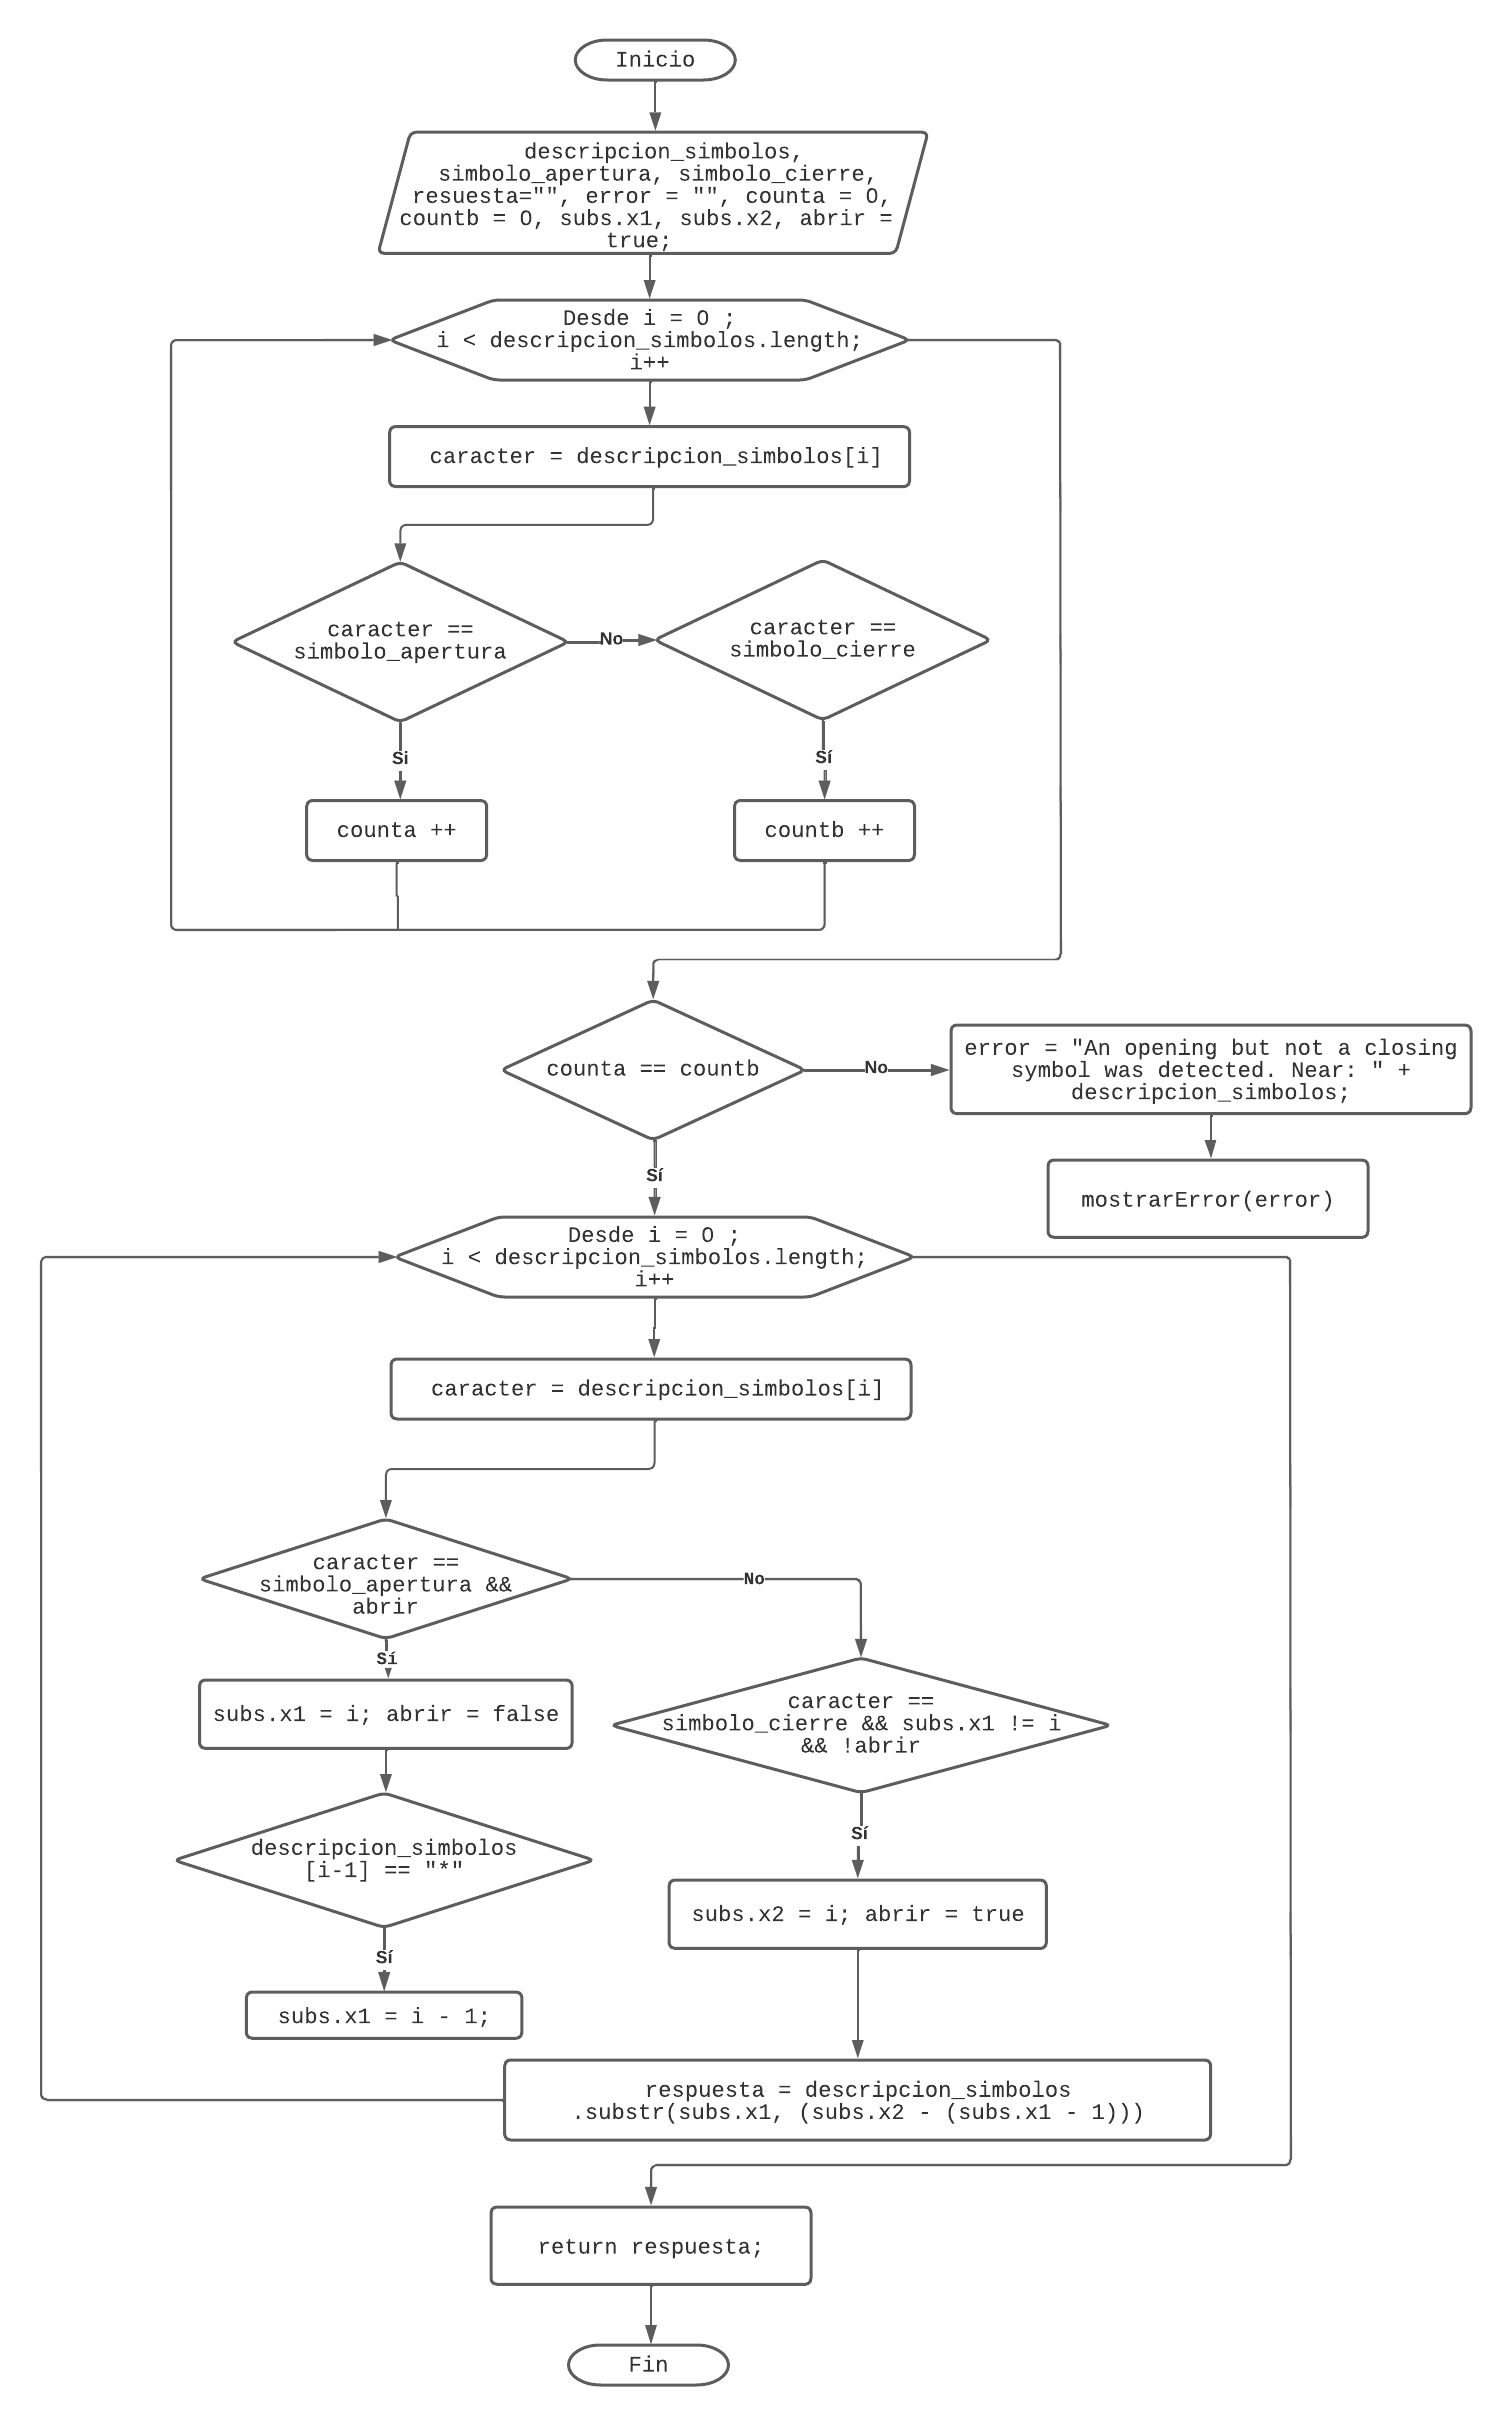
\includegraphics[width=11cm]{img/algoritmoerror.png}
	\label{fig:algoritmoerror}
	\textbf{\\ \\ ELABORADO: DÚVAL CARVAJAL SUÁREZ}
\end{figure} 

\section{Generación de código}

En la siguiente fase se desarrollaron las funciones y todos los métodos que fueron necesarios para que la librería funcione correctamente. A continuación se observan todas las variables que fueron necesarias para que todo funcione de manera correcta.
\newpage
\lstinputlisting[language=JavaScript]{codigo/variables.js}

En el siguiente bloque de código se observa la función que permite acumular los mensajes de error que pueden ocurrir al momento de interpretar las descripciones de los casos de uso. 

\lstinputlisting[language=JavaScript]{codigo/notificaciones.js}

En el siguiente bloque de código se observa una de las funciones principales para detectar los símbolos de apertura y cierre, con el objetivo de utilizar una sola función que permita identificar los símbolos que necesariamente deben ser con apertura y cierre. 

\lstinputlisting[language=JavaScript]{codigo/detectarsimbolos.js}

Para mejorar la presentación de la librería se desarrollo una aplicación web sencilla que permita utilizar de forma grafica las funciones de la misma. La aplicación web tendrá como propósito proporcionar un lugar en la web de donde descargar el script para que pueda ser usado por la comunidad de desarrolladores. Ademas de proporcionar documentación de como instalarla en otros proyectos y como utilizarla.  

\section{Ejecución de pruebas}

Para la ejecución de las pruebas, se analizo el caso de uso que fue proporcionado por el docente. Cada párrafo estaba redactado con el lenguaje de símbolos, por lo que se ingresaron las descripciones en la aplicación de demostración y los resultados fueron los siguientes:

\begin{itemize}
	\item Descripción \#1:
	\begin{lstlisting}
		This use case starts when a person *(person &-id=int) wants to register as a tutor *(tutor &-id=int [+userRegistration=Tutor]) user in the system. *¡tutor 1<[register]>n Person! \end{lstlisting}

	Interpretando el párrafo, se creo una clase denominada Tutor con sus respectivos atributos que son: \textbf{id} privado y de tipo String, los métodos que se agregaron son: \textbf{userRegistration()} publico. Ademas se realizo una relación de tipo generalización. A continuación se observa la estructura json y xml generada por la librería a partir del párrafo ingresado.
	
	\lstinputlisting[language=JavaScript]{codigo/pruebas/test01.json}
	\lstinputlisting[language=JavaScript]{codigo/pruebas/test01.xml}
	
	Para que la descripción del caso de uso pueda ser entendida por el cliente del sistema que se este desarrollando se obtiene como resultado el párrafo redactado en lenguaje natural omitiendo los símbolos y pueda ser comprendido con mayor facilidad. 
	
	\begin{lstlisting}
		This use case starts when a person wants to register as a tutor user in the system.  \end{lstlisting}
	
	Como el texto esta redactado de forma correcta la retroalimentación generada muestra mensajes exitosos:
	
	\textcolor{blue}{\textbf{information:} Description entered: This use case starts when a person *(person \&-id=int) wants to register as a tutor *(tutor \&-id=int [+userRegistration=Tutor]) user in the system. *¡tutor 1<[register]>n Person!}
	
	\textcolor{ForestGreen}{
		\textbf{success:} Successfully added attributes: id \\
		\textbf{success:} The class Person was generated successfully \\
		\textbf{success:} Successfully added attributes: id \\
		\textbf{success:} The class Tutor was generated successfully \\
		\textbf{success:} The generalization relationship between objects from: Tutor 1<>n to: Person was successfully generated. }
	
	Para verificar el funcionamiento de la retroalimentación identificando la mala escritura de las descripciones del caso de uso usando el lenguaje de símbolos, se redacto a propósito el mismo párrafo pero usando de forma incorrecta los símbolos.
	
	\begin{lstlisting}
		This use case starts when a person *(person &-id=int) wants to register as a tutor *(tutor &-id=int [+userRegistration=Tutor) user in the system. *¡tutor 1<[register]>n Person \end{lstlisting} 
	
	Observando los menajes de retroalimentación ya se identificaron que errores se están cometiendo en el uso de algunos símbolos y especificando en que lugar del texto se encuentra ese error. 
	
	\textcolor{blue}{\textbf{information:} Description entered: This use case starts when a person *(person \&-id=int) wants to register as a tutor *(tutor \&-id=int [+userRegistration=Tutor]) user in the system. *¡tutor 1<[register]>n Person!}
	
	\textcolor{ForestGreen}{
	\textbf{success:} Successfully added attributes: id \\
	\textbf{success:} The class Person was generated successfully \\
	\textbf{success:} Successfully added attributes: id}

	\textcolor{Red}{
	\textbf{error:} An opening but not a closing symbol was detected. => begin: [, end: ]. Near: *(tutor \&-id=int [+userRegistration=Tutor)}

	\textcolor{ForestGreen}{\textbf{success:} The class Tutor was generated successfully }
	
	\textcolor{Red}{
	\textbf{error:}  An opening but not a closing symbol was detected. => begin: ¡, end: !. Near: This use case starts when a person *(person \&-id=int) wants to register as a tutor *(tutor \&-id=int [+userRegistration=Tutor) user in the system. *¡tutor 1<[register]>n Person}

	Utilizando la aplicación web de demostración, se logra observar ene la figura \ref{fig:prueba01} el diagrama de clases creado a partir de la estructura json o xml que la librería proporciona de forma automática. 
	
	\begin{figure}[h!]
		\caption{Diagrama de clases generado por la aplicación web de demostración usando la librería de armadillo.js}
		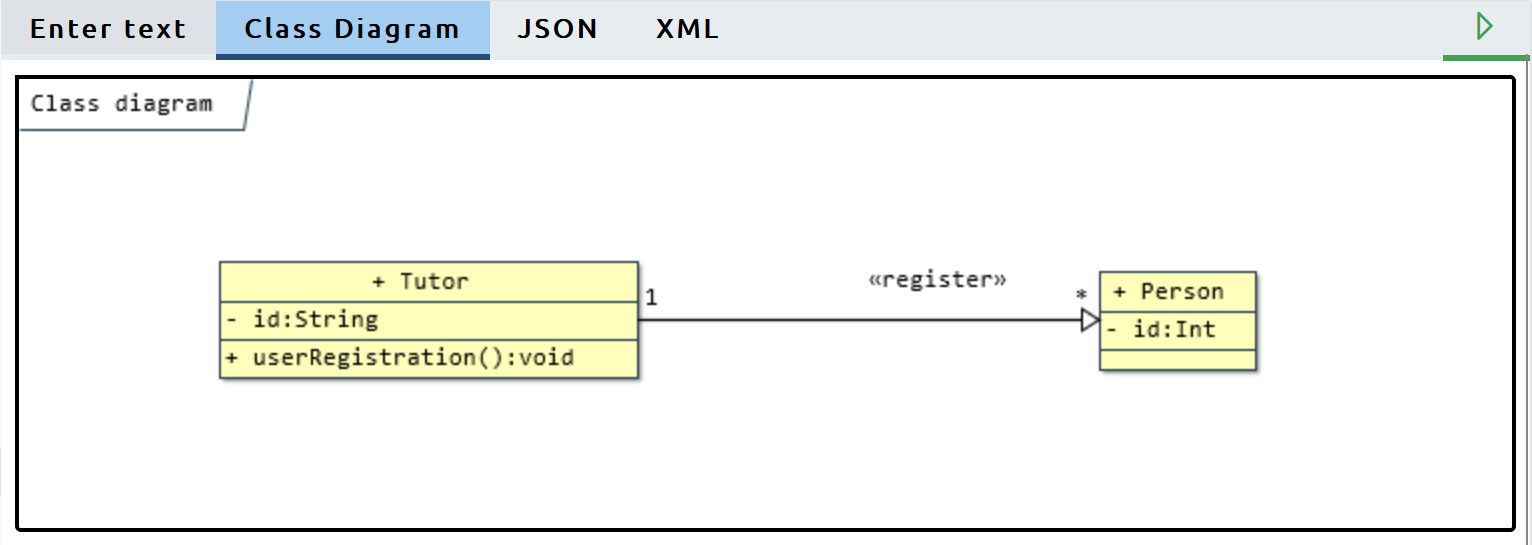
\includegraphics[width=15cm]{img/prueba01.png}
		\label{fig:prueba01}
		\textbf{\\ ELABORADO: DÚVAL CARVAJAL SUÁREZ}
	\end{figure}
	
\end{itemize}

\section{Evaluación con sistemas de información}

Para la ejecución de la fase final de la metodología se revisaron varios proyectos de titulación realizados por estudiantes de la Universidad Técnica Estatal de Quevedo. Se analizaron los sistemas desarrollados reescribiendo las descripciones de los casos de uso utilizando el lenguaje de símbolos. 

\begin{table}[h!]
	\caption{Descripción del caso de uso para iniciar sesión.}
	\begin{tabular}{| p{3cm} | p{11cm} |}
		\hline
		\textbf{Caso de uso:} & Iniciar sesión \\ \hline
		\textbf{Actores:} & Cuidador \\ \hline
		\textbf{Propósito:} & Ingresar a la interfaz principal de la aplicación \\ \hline
		\textbf{Resumen:} & 
		Permite identificar las credenciales del usuario que intenta ingresar al sistema, de esa forma verificar el tipo de usuario que ingresa. \\ \hline
		\textbf{Tipo:} & Primario \\ \hline
		\multicolumn{2}{ |c| }{\textbf{Flujo normal}} \\ \hline
	\end{tabular}
	\begin{tabular}{| p{7cm} | p{7cm} |}
		1. Este caso de uso inicia el actor cuidador pretende ingresar al sistema. & \\ \hline
		2. Ingresa al sistema. & \\ \hline
		& 3. Muestra la interfaz donde se necesitan ingresar las credenciales de acceso que son un usuario y contraseña. \\ \hline
		4. Ingresa sus credenciales de acceso que son el usuario y contraseña. & \\ \hline
		& 5. Verifica que el usuario y contraseña se encuentren registrados en la aplicación. \\ \hline
		& 6. El sistema da acceso a la interfaz de inicio de la aplicación. \\ \hline
		\multicolumn{2}{ |c| }{\textbf{Flujos alternos}} \\ \hline
	\end{tabular}
	\begin{tabular}{| p{7cm} | p{7cm} |}
		& 5.1 Si el usuario y contraseña no existen en el sistema, se mostrara un mensaje de dialogo notificando lo sucedido. Retornar al paso 4. \\ \hline
	\end{tabular}
	\textbf{ \\ ELABORADO: DÚVAL CARVAJAL SUÁREZ}
\end{table}
